\chapter{بررسی روش آرنج برای تخمین تعداد خوشه‌ها}

\section{آزمایش نخست: داده‌ی \lr{D1}}

آزمایش برای $k=2,\ldots,10$ و گراف ۱۲-نزدیک‌ترین همسایه اجرا شد و هزینه برابر
$100936.0647$ باقی ماند. در نتیجه هیچ منحنی آرنج معناداری ساخته نشد.

\section{آزمایش دوم: داده‌ی \lr{Gisette}}

برای داده‌ی \lr{Gisette} با گراف ۸۰-نزدیک‌ترین همسایه، الگوریتم به همه‌ی
مقادیر درخواستی رسید. نتایج تابع هدف در جدول \ref{tab:gisette-elbow} آمده است.

\begin{table}[H]
\centering
\caption{هزینه‌ی \lr{GLKM} روی \lr{Gisette} برای مقادیر مختلف $k$}
\label{tab:gisette-elbow}
\begin{tabular}{cccccccccc}
\toprule
$k$ & 2 & 3 & 4 & 5 & 6 & 7 & 8 & 9 & 10\\
\midrule
$\Phi/10^7$ & \lr{2.586} & \lr{2.580} & \lr{2.574} & \lr{2.568} & \lr{2.563} & \lr{2.557} & \lr{2.552} & \lr{2.546} & \lr{2.541}\\
\bottomrule
\end{tabular}
\end{table}

روش فاصله از وتر $k=5$ را انتخاب کرد؛ بااین‌حال کاهش هزینه تقریباً خطی است. همچنین معیارهای \lr{ACC} و \lr{NMI} در
$k=2$ بهتر بودند. بنابراین $k=5$ بیشتر محصول حساسیت هندسی روش eblow
است.

\begin{figure}[H]
\centering
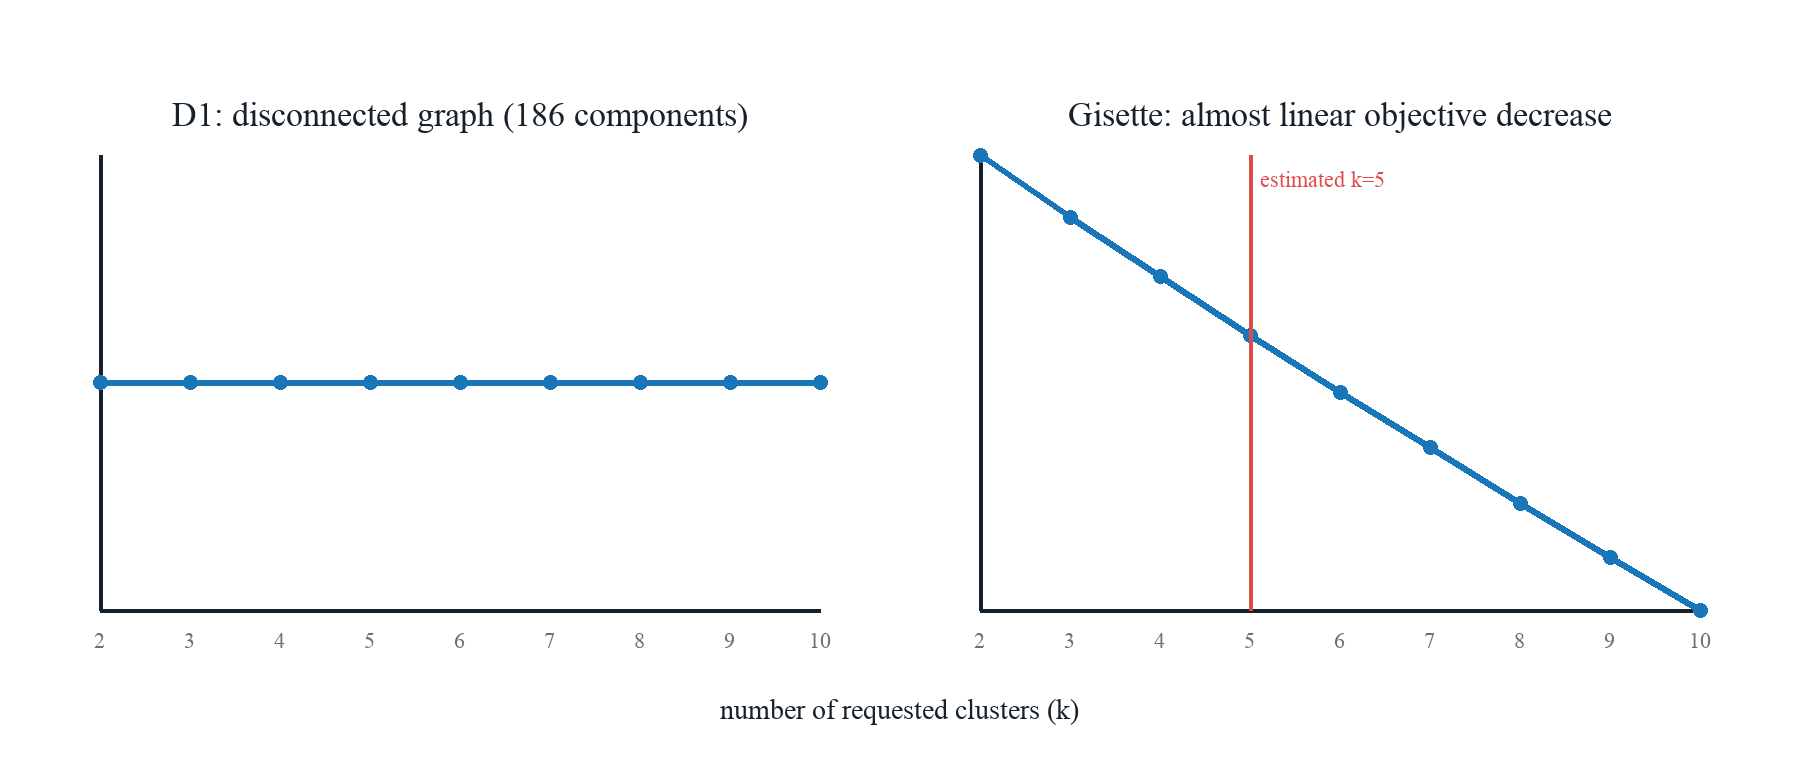
\includegraphics[width=\textwidth]{Figures/elbow_results.png}
\caption{دو شکست روش آرنج}
\label{fig:elbow-results}
\end{figure}

\section{جمع‌بندی آزمایش}

روش آرنج در شکل فعلی جایگزین مطمئنی برای ورودی $k$ نیست.هرچند بر اساس یافته‌های فعلی می‌توان در آینده مسیر توسعه بهتری را در پیش گرفت.

